\subsection{Modelling}

\begin{frame}{Modelling}
  \begin{block}{Antennas}
      Describing the movement of the antennas when the UA is flying far away from the GS. 
    \end{block}

  \begin{figure}[H]
    \centerline{
    \subfigure[UAS Map]{
    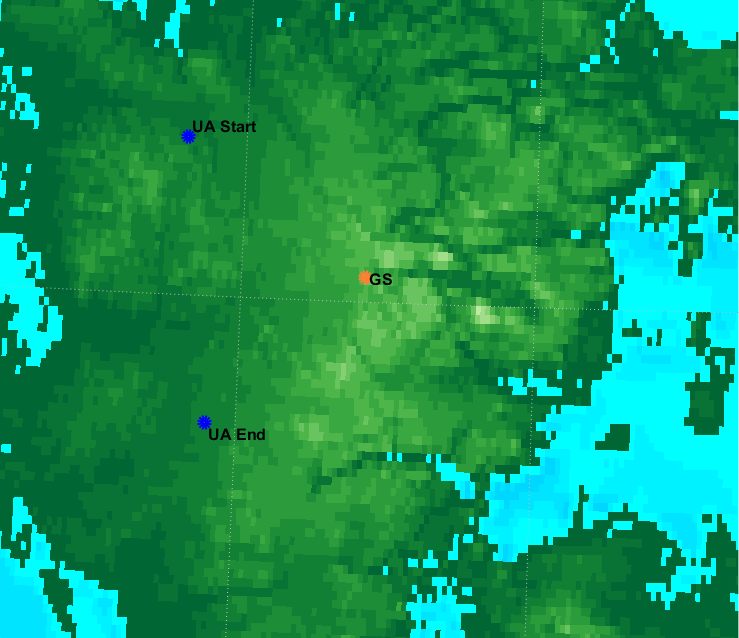
\includegraphics[scale=0.3]{figures/s1_zoom.png}}
    \subfigure[Distance between UA and GS]{
    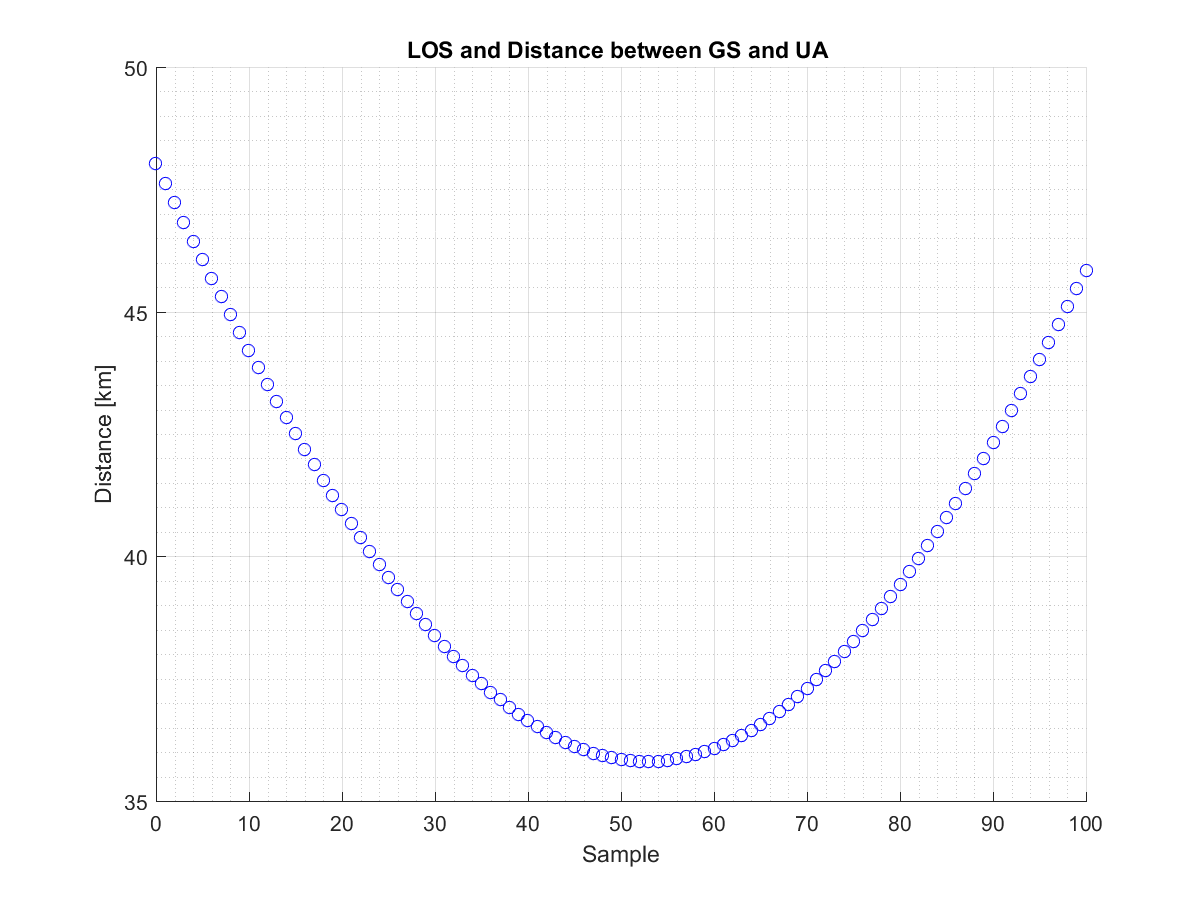
\includegraphics[scale=0.31]{figures/s1_los.png}}}
  \end{figure}
\end{frame}

\begin{frame}{Modelling}
  \begin{block}{Optimal Angle}
      Describing the movement of the antennas when the UA is flying far away from the GS. 
    \end{block}

  \begin{figure}[H]
    \centerline{
    \subfigure[UAS Map]{
    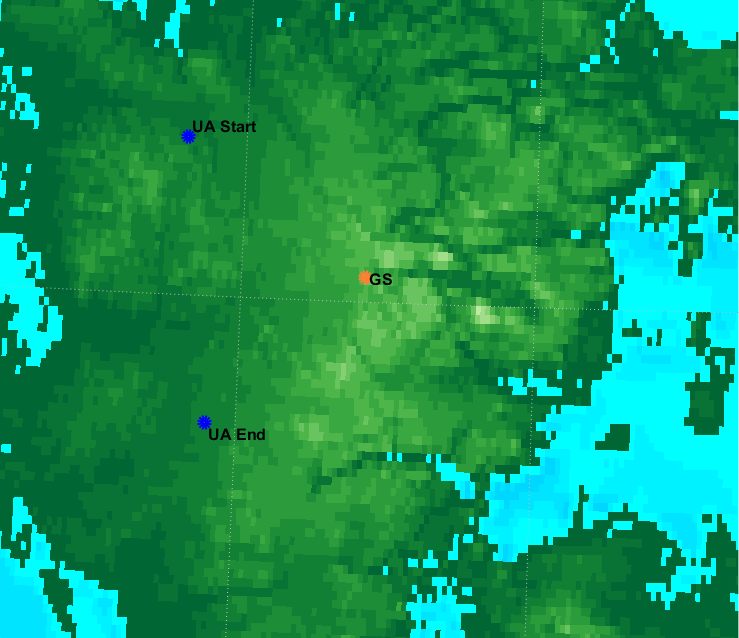
\includegraphics[scale=0.3]{figures/s1_zoom.png}}
    \subfigure[Distance between UA and GS]{
    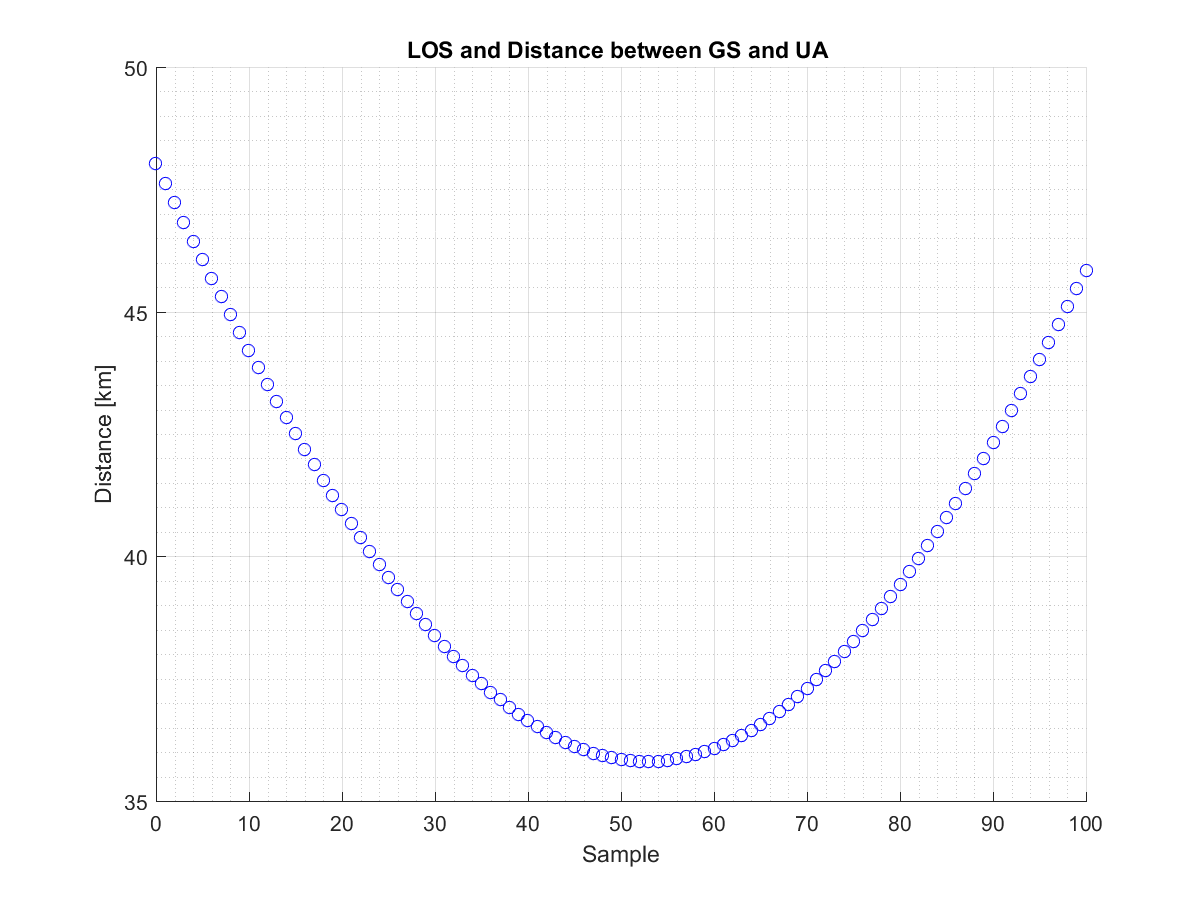
\includegraphics[scale=0.31]{figures/s1_los.png}}}
  \end{figure}
\end{frame}

\begin{frame}{Modelling}{}

  \begin{block}{Moving Angle System (MAS)}

  \end{block}

\end{frame}
